\documentclass{standalone}
\usepackage{pgfplots}
\usepackage{xcolor}
\usepgfplotslibrary{statistics}
\pgfplotsset{compat=1.17}

% Auburn colors
\definecolor{auburnorange}{RGB}{232, 119, 34}
\definecolor{auburnblue}{RGB}{12, 35, 64}
\definecolor{lightgray}{gray}{0.9}

\begin{document}
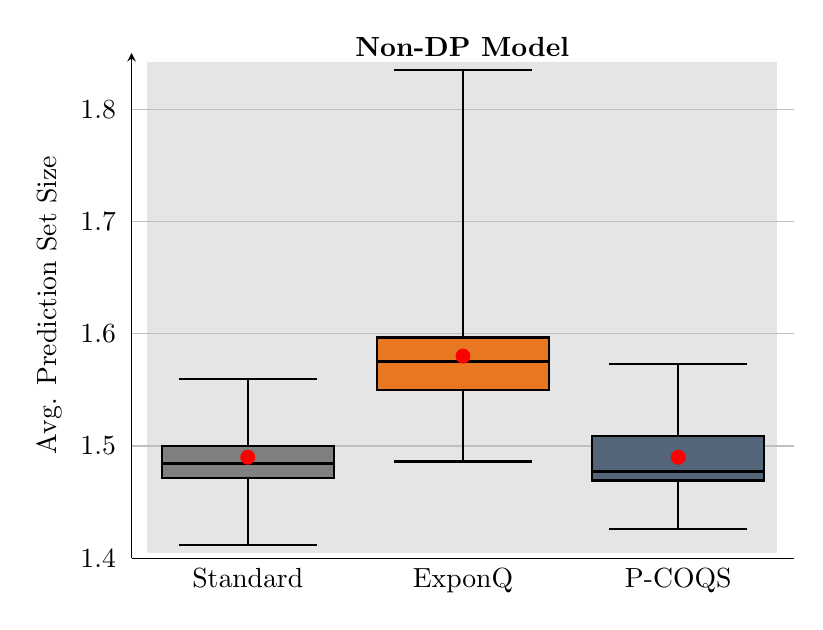
\begin{tikzpicture}

% Background for non-DP models
\fill [lightgray] (0.2,0.07) rectangle (8.2,6.3);

\begin{axis}[
    boxplot/draw direction=y,
    ylabel={Avg. Prediction Set Size},
    xtick={1,2,3},
    xticklabels={
        {Standard},
        {ExponQ},
        {P-COQS}
    },
    x tick label style={align=center},
    ymin=1.4, ymax=1.85,
    width=10cm,
    height=8cm,
    ymajorgrids,
    axis x line*=bottom,
    axis line style={-},
    axis y line=left,
    tick style={draw=none},
    enlarge x limits=0.05,
    boxplot/every box/.style={draw=black, thick, solid},
    boxplot/every whisker/.style={black},
    boxplot/every median/.style={black, very thick},
]

% Standard (Non-DP)
\addplot+[
    draw=black, solid, thick,
    fill=gray,
    boxplot prepared={
        lower whisker=1.4120,
        lower quartile=1.4718,
        median=1.4843,
        upper quartile=1.5002,
        upper whisker=1.5596
    },
] coordinates {};

% ExponQ (Non-DP)
\addplot+[
    draw=black, solid, thick,
    fill=auburnorange,
    boxplot prepared={
        lower whisker=1.4862,
        lower quartile=1.5502,
        median=1.5750,
        upper quartile=1.5966,
        upper whisker=1.8348
    },
] coordinates {};

% P-COQS (Non-DP)
\addplot+[
    draw=black, solid, thick,
    fill=auburnblue!70,
    boxplot prepared={
        lower whisker=1.4264,
        lower quartile=1.4692,
        median=1.4770,
        upper quartile=1.5088,
        upper whisker=1.5732
    },
] coordinates {};

% Red mean dots
\addplot[
    only marks,
    mark=*,
    mark size=2.5pt,
    red
] coordinates {
    (1, 1.49)
    (2, 1.58)
    (3, 1.49)
};

\end{axis}

\node at (4.2,6.5) {\textbf{Non-DP Model}};

\end{tikzpicture}
\end{document}
